\subsection{Sprint 5}
\subsubsection{Sprint start}

\subsubsection{Sprint burndown}



\begin{figure}[H]
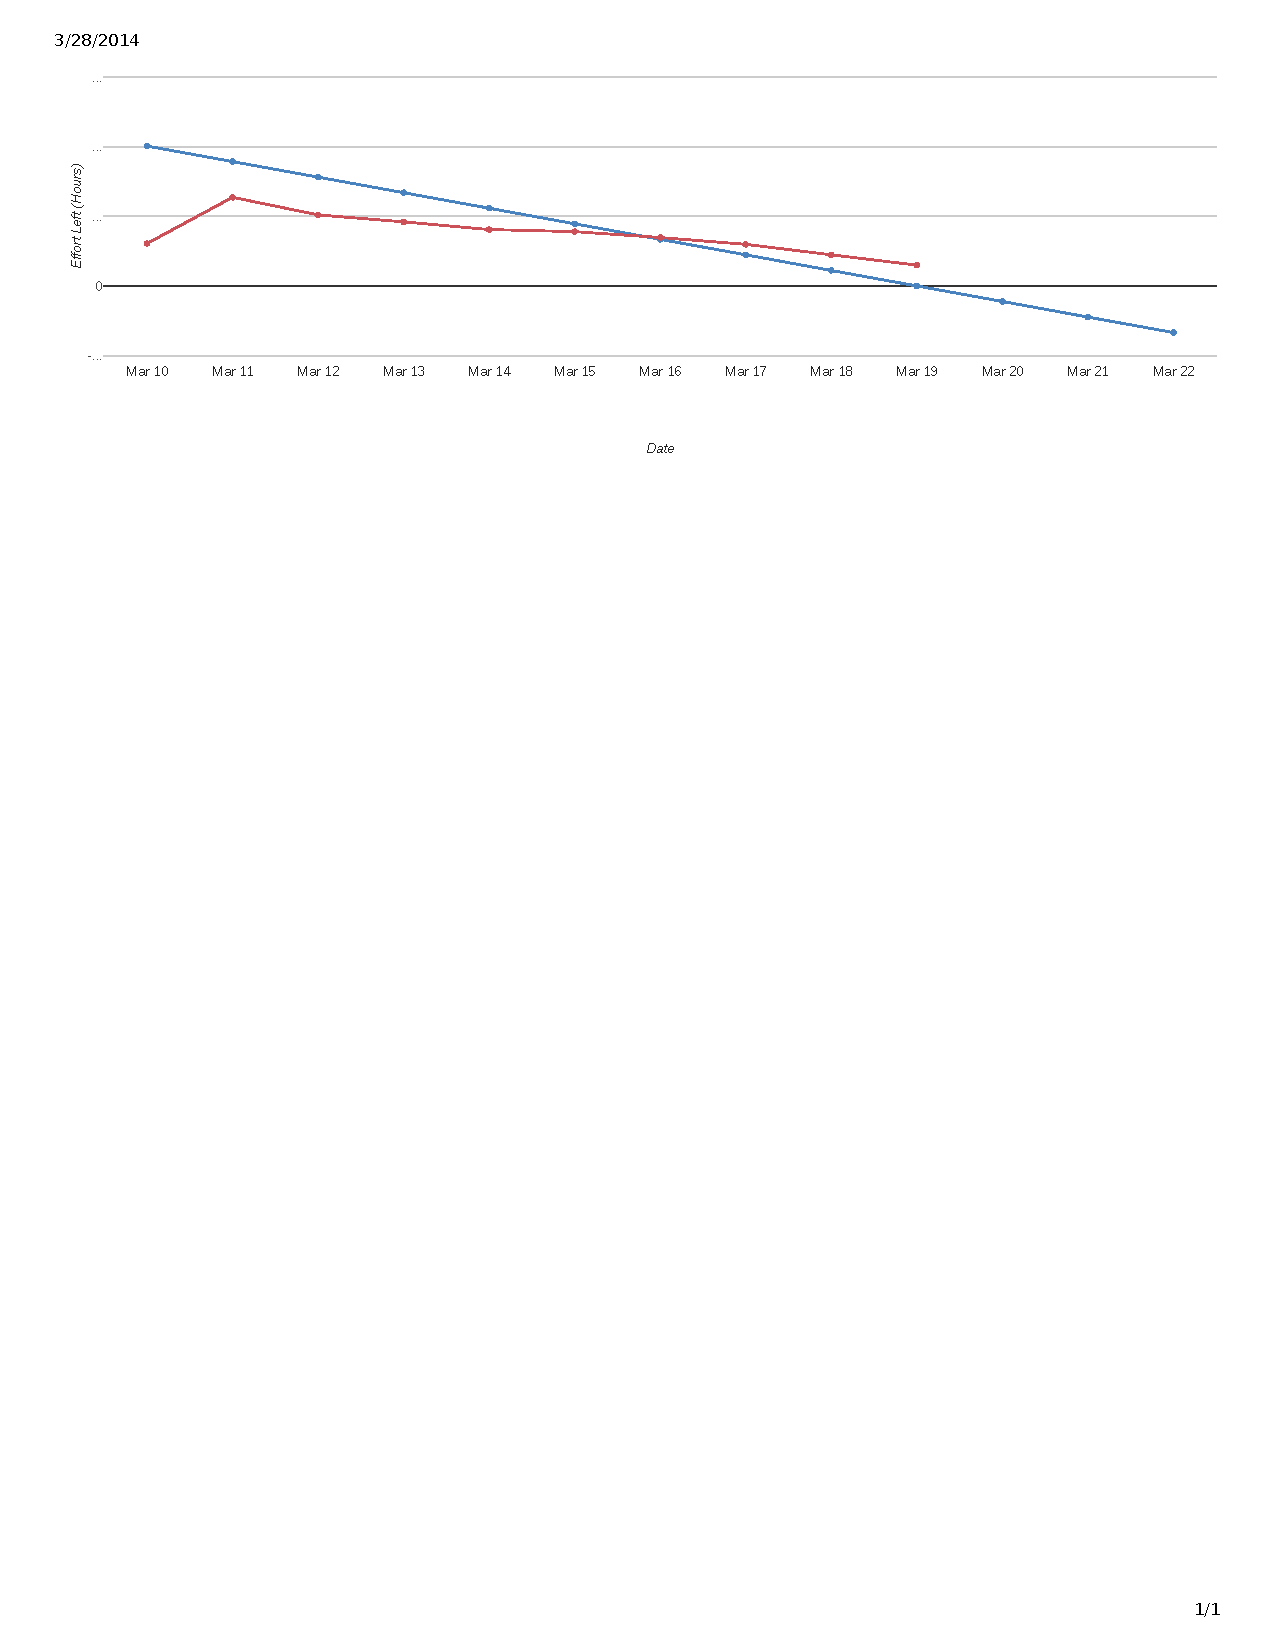
\includegraphics[width=\textwidth, trim= 1cm 21cm 1cm 1cm, clip=true]{ch/projectManagement/fig/burndown4.pdf}
\caption{Sprint 5 burndown chart}
\label{fig:sprint5burndown}
\end{figure}

\subsubsection{Sprint backlog}



\begin{table}[H]
	\begin{tabular}{|l|p{7cm}|p{2.2cm}|p{1.5cm}|p{1.5cm}|}%
		\hline \bfseries User story & \bfseries Details & \bfseries Hours\newline estimated & \bfseries Hours spent & \bfseries Hours left
		\csvreader[head to column names]{ch/projectManagement/sec/sprints/sprint5/userstories.csv}{}% use head of csv as column names
		{\\\hline \id & \title & \estimated & \spent & \left} \\\hline% specify your coloumns here
	\end{tabular}
    \caption{Sprint 3 backlog}
\end{table}


\subsubsection{Sprint end}

\subsubsection{Review of main responisbility areas}
\label{sec:unbalancedWorkload}
During this sprint, the team evaluated whether the use of the team's available resources actually were fully exploited. We acknowledged that our current Scrum master, Per Øyvind, had the best control of the development environment, which in turn lead to that the workload he got due to his position as Scrum master and his level of expertise, was too great. We therefore decided that Lars Erik, which previously was our deputy project leader, was the best fit for our new Scrum master.

We also discussed whether the position ''Project leader'' actually was necessary, as it conflicted with one of the principles in Scrum. The team decided that we in fact thought the position was necessary, as the project leader and Scrum master simply distributed the Scrum master's traditional tasks between them. The main difference would be that the project leader would handle the administrative tasks, such as room booking for meetings and work sessions, and handle customer relations, while the Scrum master would handle the project administrative tasks, such as moderating the Scrum meetings, adding tasks to the backlog and Yodiz, and generate burndown charts.